\documentclass[pdftex,12pt,a4paper]{article}

\usepackage[utf8]{inputenc}
\usepackage[T1]{fontenc}
\usepackage[frenchb]{babel}
\usepackage{color}
\usepackage[usenames,dvipsnames,svgnames,table]{xcolor}
\usepackage{lmodern}
\usepackage{lastpage}
\usepackage[pdftex]{graphicx}
\usepackage{fancyhdr}
\usepackage{geometry}
\usepackage{url}
\usepackage[colorlinks=true,urlcolor=blue,linkcolor=blue]{hyperref}
\usepackage{fancyvrb}
\usepackage{multicol}


\geometry{top=3cm, bottom=2.5cm, left=2cm, right=2cm}
\setcounter{tocdepth}{3}

%%%%%%%  VARIABLES     %%%%%%%%%%%%%%%%%%%%%%%%%%%%%%%%%%%%%
\newcommand{\docauthor}{
            Maxime \textsc{Pauvert} 
     		\& David \textsc{Perrai} \\
                       
 }
\newcommand{\doctitle}{ScalaTextEditor}
%%%%%%%%%%%%%%%%%%%%%%%%%%%%%%%%%%%%%%%%%%%%%%%%%%%%%%%%%%%%

%%%%%%%   MAKE TITLE   %%%%%%%%%%%%%%%%%%%%%%%%%%%%%%%%%%%%%
\author{\docauthor}
\title{\doctitle}
\date{\today}
%%%%%%%%%%%%%%%%%%%%%%%%%%%%%%%%%%%%%%%%%%%%%%%%%%%%%%%%%%%%

%%%%%%  EN-TETE / PIED-PAGE %%%%%%%%%%%%%%%%%%%%%%%%%%%%%%%%
\pagestyle{fancy}
\fancyhead{}
\fancyfoot{}
\lhead{\leftmark}
\rhead{\doctitle}
\rfoot{\thepage/\pageref{LastPage}}
\lfoot{Génie logiciel}
\renewcommand{\footrulewidth}{0.5pt}
\renewcommand{\headrulewidth}{0.5pt}
%%%%%%%%%%%%%%%%%%%%%%%%%%%%%%%%%%%%%%%%%%%%%%%%%%%%%%%%%%%%

%%%%%%  SETTING COLOR %%%%%%%%%%%%%%%%%%%%%%%%%%%%%%%%%%%%%%
%\definecolor{key}{rgb}{0.6,0,0.6}
%\definecolor{bck}{rgb}{0.92,0.92,0.92}
%\definecolor{comment}{rgb}{0.5,0.5,0.5}
%\definecolor{string}{rgb}{0,0.5,0}
%\definecolor{number}{rgb}{0,0.5,0.5}
%%%%%%%%%%%%%%%%%%%%%%%%%%%%%%%%%%%%%%%%%%%%%%%%%%%%%%%%%%%%

%%%%%% SETTING %%%%%%%%%%%%%%%%%%%%%%%%%%%%%%%%%%%%%%%%%%%%%
%\lstset{
%language=clean,
%basicstyle=\fontfamily{lmtt} \small,
%numbers=left,
%numbersep=7pt,
%numberstyle=\small,
%showspaces=false,
%showtabs=false,
%tabsize=4,
%xleftmargin=20pt,
%xrightmargin=20pt,
%morekeywords={},
%%backgroundcolor=\color{bck},
%commentstyle=\color{comment},
%keywordstyle=\color{string},
%breaklines=true
%}

\newcommand{\name}[1]{\textsc{#1}}
\newcommand{\commande}[1]{\texttt{#1}}

\fvset{frame=single,fontsize=\scriptsize,xleftmargin=2cm,xrightmargin=2cm}

\renewcommand{\FrenchLabelItem}{\space\textbullet}

\newcommand{\HRule}{\rule{\linewidth}{0.5mm}}

\newcommand{\reffig}[1]{(Figure \ref{#1})}

\setlength{\parskip}{1ex plus .8ex minus .8ex}
\setlength{\parindent}{.8em}
\linespread{1.3}
%%%%%%%%%%%%%%%%%%%%%%%%%%%%%%%%%%%%%%%%%%%%%%%%%%%%%%%%%%%%

\begin{document}

  \begin{titlepage}
    \begin{center}
      %%\includegraphics[width=15cm]{./cellule.jpg}~\\[3cm]

      \HRule \\[0.5cm]
      \textsc{\LARGE \doctitle \\[0.5cm]}
      \textbf{\Large Rapport Mini-Editeur \\[0.5cm]}
      \HRule \\[1.25cm]

		\docauthor
      ~\\[1.0cm]
      \today

      \vfill{}
      
    \end{center}
  \end{titlepage}

\tableofcontents
\setcounter{page}{1}
\newpage
	

  
	\begin{abstract}
    Dans le cadre du cour de Génie logiciel il nous a été demandé de mettre en oeuvre un projet de mini-editeur de texte. Ce projet a pour but de mettre en place les connaissances apprises durant le cours. Ainsi nous avons développé le mini-editor àà l'aide d'une modélisation UML pour la conception en amont et au cour du développement, avec la mise en place de patrons de conception. Nous vous présenterons le programme et ses fonctionnalités puis la conception de l'architecture  à travers les diagrammes UML et enfin nous expliciterons les différents patrons et leurs rôles dans le programme ainsi que certains choix d'implémentation.
    \end{abstract}
    
    \section{Présentation de ScalaTextEditor}
    	ScalaTextEditor est un mini-editeur de texte en ligne de commande, l'utilisateur a comme actions disponible:\\
        \begin{itemize}
        	\item Ecriture de texte.
            \item Déplacement du curseur.
            \item Supression du texte.
            \item Copie dans un presse-papier d'une sélection effectué sur le texte.
            \item Collage d'une sélection du presse-papier. 
            \item Revenir en arrière sur les dernières actions effectués. 
		\end{itemize}
   
        

    	\section{Analyse du domaine}
    Pour concevoir cette éditeur de texte nous avons identifié dans un premier temps les concepts principaux du programme :
    
    	\begin{enumerate}
        	\item  l'espace de travail de l'utilisateur est le coeur de l'application où sont éxécutées des actions.
            \item  un curseur simple permettant à l'utilisateur de ce déplacer dans le texte 
            \item un curseur de selection permettant de sélectionner un passage du texte
            \item le presse-papier permettant à l'utilisateur d'enregistrer une sélection 
            \item les commandes que l'utilisateur pourra effectuer (écriture, effacement, copie, collage\dots) \\
        
        \end{enumerate} 
       
  A l'aide de cette analyse nous avons extrait les différentes classes composant le système. Pour le comportement et l'architecture de notre programme nous avons utilisé différents patrons de conception. (voir l'architecture générale sur le projet papyrus).
        \newpage
         
         \section{Conception détaillée}
 
      %%%%% patron de conception observer %%%%  
   \subsection{Patron de conception: Observer} 
      Le patron de l'observer sert dans ce cadre à mettre à jour "l'espace de travail" (\emph{Workspace}) de l'utilisateur (\emph{UI}) lorsqu'il effectue des modifications dans le texte. La classe UI est donc un observeur qui observe la classe  observable workspace qui la notifie lors de son changement.\\
      
      
       \begin{figure}[htb]
        	\begin{center}
        	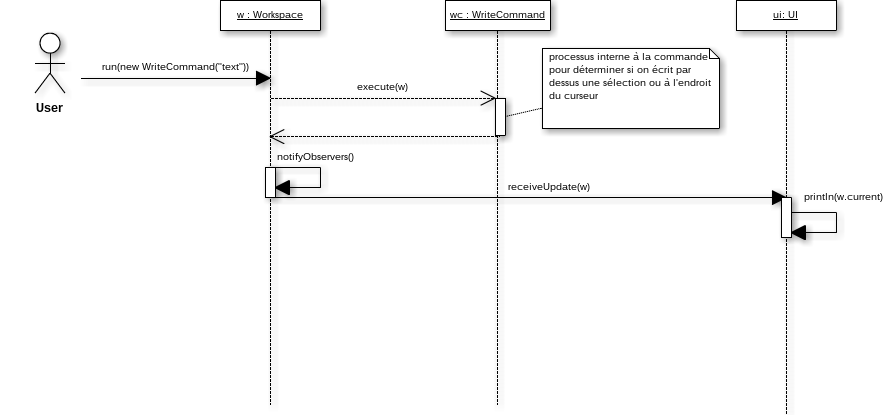
\includegraphics[width=1.0\textwidth]{./seqObserver.png}\caption{diagramme de Séquence de l'observer}
             \end{center}
      	\end{figure}
        
Dans ce diagramme de séquence l'utilisateur execute une commande d'écriture (\emph{WriteCommand}) en remplacement d'une sélection ou à l'endroit de son curseur. Le workspace est alors mis à jour et contient désormais le texte écrit par l'utilisateur. L'espace de travail met ensuite à jour l'interface de l'utilisateur en lui notifiant de son changement.      
        
        
          \begin{figure}
        	\begin{center}
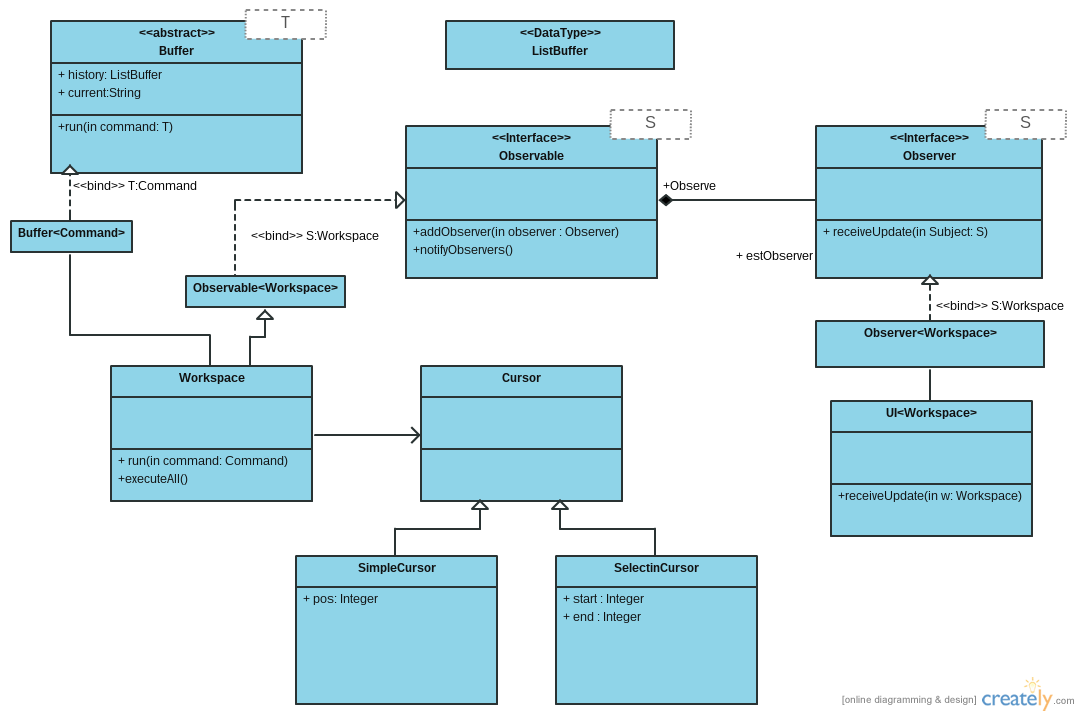
\includegraphics[width=1.0\textwidth]{./obsgl.png}\caption{diagramme de classe de l'observeur}
             \end{center}
      	\end{figure}
        
        	\newpage

         
   	 %%%%% patron de conception commande %%%%        
   \subsection{Patron de conception: Commande}

Le patron de conception commande est utilisé dans ce contexte pour l'éxecution des actions (les commandes) de l'utilisateur à partir de "son espace de travail" (\emph{workspace}). Il sert entre aute à conserver une sélection copier dans le presse-papier (\emph{clipboard}) lors de l'éxecution d'une commande de type copie ou encore à coller un contenu du presse-papier à un endroit du texte (par dessus une sélection ou à la position du curseur) 
        
        \begin{figure}[htb]
        	\begin{center}
        	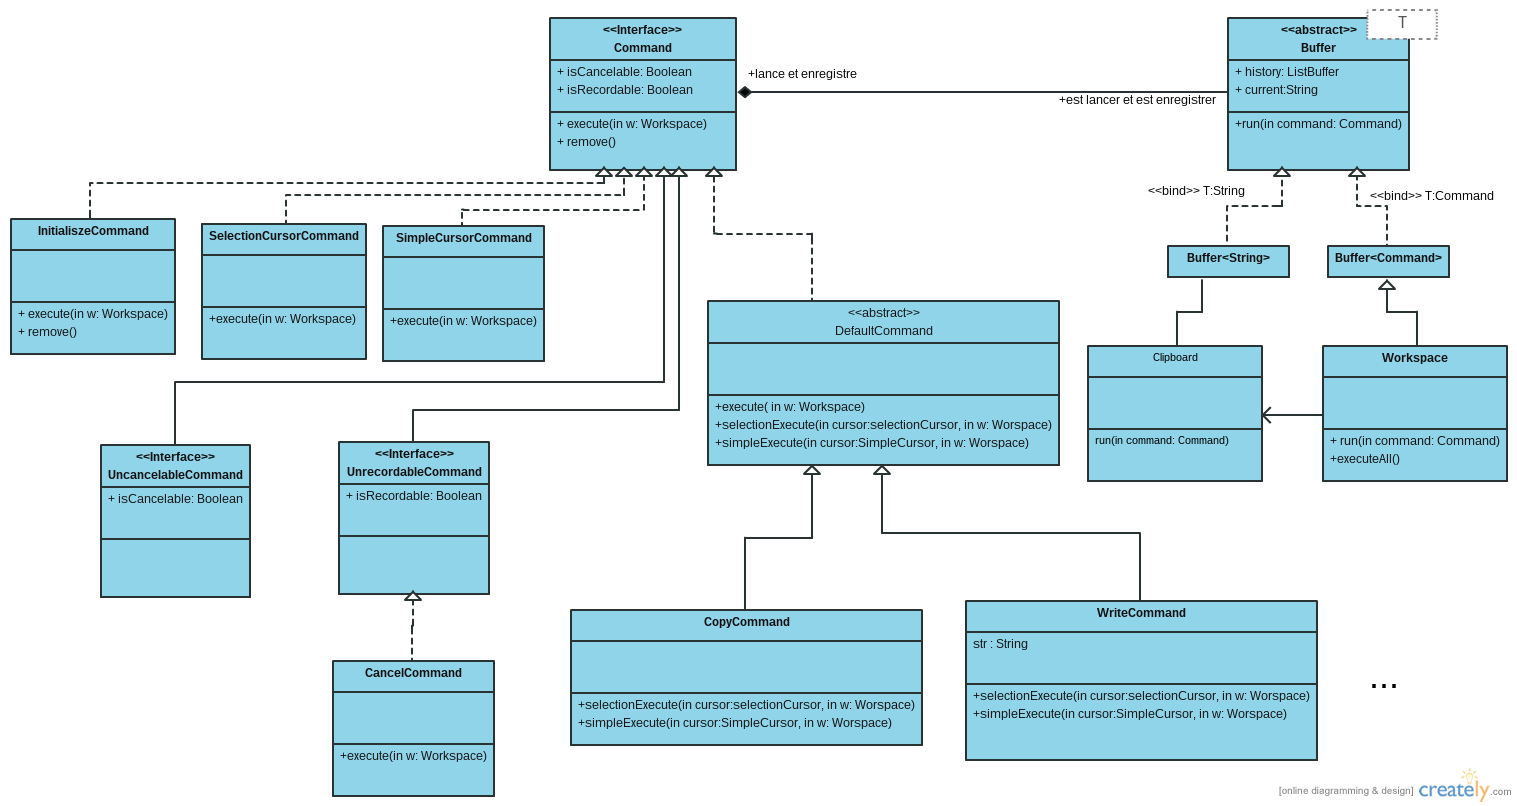
\includegraphics[width=1.1\textwidth]{./commandGl.png}\caption{diagramme de classes du patron Commande}
             \end{center}
      	\end{figure}
        
 A noter que les "\dots" représentent d'autres commandes (la commande \emph{couper}, \emph{supprimer}, \emph{coller})  mais qui n'apportent rien dans la modélisation et pour la compréhension. Cependant ces classes sont présentes dans le diagramme de l'architecture générale du projet papyrus.
 		\newpage
  %%%%% patron de conception composite %%%%  
    \subsection{Patron de conception: Composite}
        Le patron de conception composite permet de composer les commandes entre elles car certaines commandes sont contruites à partir d'autres commandes. 
         %% photo diagramm de sequence + diagramm de classe 	
   		\begin{figure}[htb]
        	\begin{center}
        	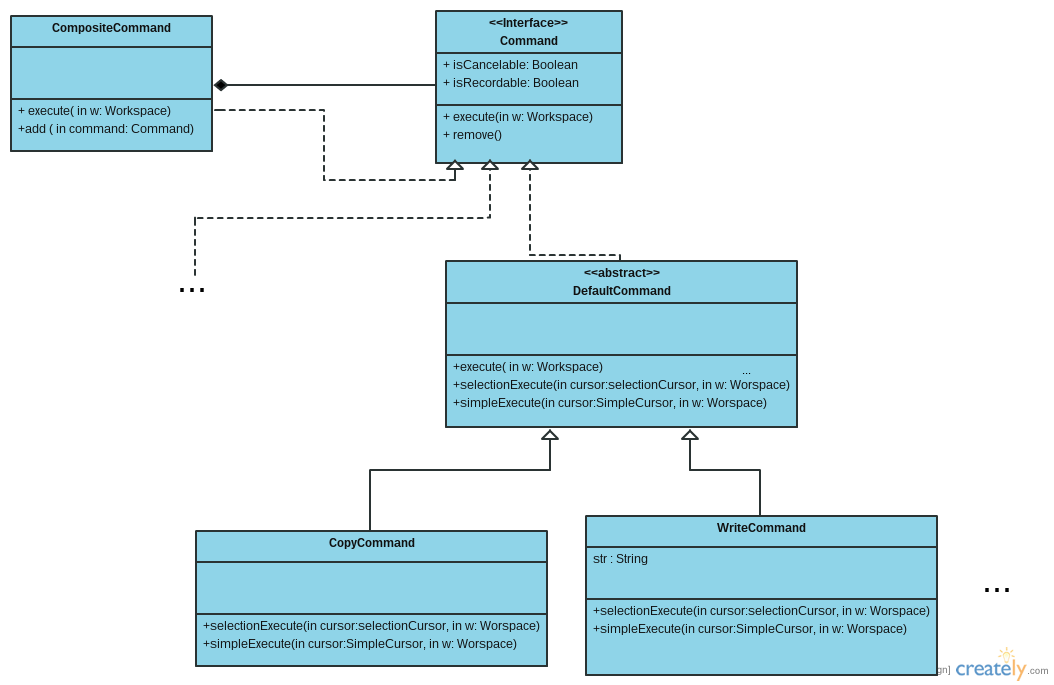
\includegraphics[width=1.1\textwidth]{./CompositeGl.png}\caption{diagramme de classes du patron composite}
             \end{center}
      	\end{figure}
        
Comme pour le diagramme précédent la présence des "\dots" représentent d'autres classes qui n'apportent rien à la compréhension.
 
       \newpage
      \section{Choix d'implémentation}
      
 	\subsection{Commande d'initialisation}
       La commande \emph{InitializeCommand} est une commande particulière. Elle permet d'initialiser  le système en mettant le curseur à une position initialise de 0, c'est à dire au début d'une ligne. En outre elle initialise le texte courant de l'espace de travail à vide. Cette commande est executé à l'instanciation de l'espace de travail (\emph{Worspace}).Si elle est réexcuté, le texte courant sera réinitialisé et le curseur sera replacé en début de ligne. La commande sera alors conservée dans l'historique des commandes et pourra être annulée. Du fait qu'elle place le curseur en début de ligne il n'est pas possible d'executé une commande de suppression (\emph{DeleteCommand}) dans le cas échéant une exception sera levé pour prévenir l'utilisateur.
        
     enregistrable\subsection{Commande d'annulation}
 	La commande d'annulation est une autre commande particulière. Elle permet d'annuler une ou plusieurs commandes executées au-paravant et ce jusqu'à la dernière commande enregistrée dans l'historique des commandes. Etant une commande qui annule une autre commande elle ne doit pas être enregistrable dans l'historique, dans le cas échéant on ne pourrait annuler que la dernière commande qui serait remplacée dans l'historique par une commande annulée qui serait elle même remplacée par une commande annulée dans le cas d'une autre annulation.\\ 
    
    Pour évité ce comportement nous avons mis en place d'un attributs booléen (isRecordable)  qui sera interprété lors de l'execution de commandes pour éviter l'enregistrement et donc une annulation d'une commande d'annulation. \\
    
    Dans un premier temps nous avions aussi rajouté un autre attribut booléen pour géré l'annulation (isCancellable) cependant nous avons déterminé que si une commande n'était pas enregistrée dans l'historique elle ne pourrait pas être annulée car seule les commandes présentent dans l'historique peuvent l'être. Le comportement obtenu avec l'attribut isRecordable inclue  donc le comportement de l'attribut isCancellable. Nous avons tout de même conservée l'attribut dans le cas ou l'on souhaiterai rajouter une commande qui serait enregistrable dans l'historique mais qui ne serait pas annulable.
    
     
\end{document}


